\documentclass[11pt,a4paper]{article}
\usepackage[utf8]{inputenc}
\usepackage{amsmath}
\usepackage{amsfonts}
\usepackage{amssymb}
\usepackage{fullpage}
\usepackage{graphicx}
\begin{document}
\begin{center}
{\Huge New Ideas: Giri}
\end{center}

\section{Space Wake studies}
The vacuum that has been generated by the best vacuum generators on ground have gone only go upto a particular level of purity. However, we can use the naturally available vacuum in space. The problem is that the vacuum available in LEO is not very pure. High purity vacuum can be obtained in higher orbits, but it is not feasible to reach those with CubeSats. This idea is that we can have a CubeSat with an inflatable disk-like structure, orbit around the earth in LEO. Studies show that this produces very highly pure vacuum in it's wake. We can have the other CubeSats follow in this wake to conduct any required experiments. Possible applications are: Understanding atmospheric density distribution, understanding wake patterns of satellites, producing highly pure materials etc. Formation flying is useful for this mission, it can be performed in LEO and 4-5 CubeSats might be ideal for it (depending on the application). A representational image has been given below. 

\begin{figure}[!ht]
\begin{center}
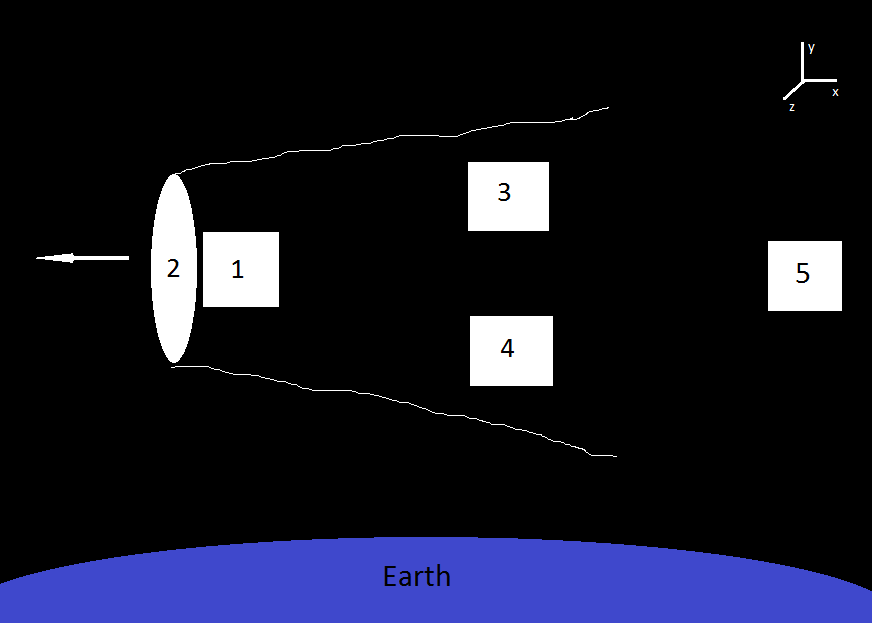
\includegraphics[scale=0.6]{wake_test.png}
\end{center}
\end{figure}

The first or leader CubeSat in the above figure is denoted by 1. The oval denoted by 2 in the figure is the inflatable structure. The earth is shown below and the direction of motion is also indicated. CubeSats 3, 4 and 5 will follow in approximately that formation. The white line extending from the end of the inflatable structure is just a representation of the wake created (Note: This may not be how the wake actually looks).  Each of the CubeSats will have a sensor in front of it which can measure the drag felt by it (I am not yet sure what this sensor would be). CubeSat 3 and 4 would feel less drag as they are in the immediate wake of the leader. CubeSat 5 would feel much more than 3 and 4 as it is farther away. Thus using the differential drag measurements of the leader and CubeSats 3 and 4, a density model of the atmosphere can be generated. A study on the how much drag is felt by CubeSat 5 while varying the distance between the leader and CubeSat 5 can also be done. We can also have additional CubeSats along the z axis using which we can measure the 3D variations. 

\section{Open source CubeSat Testbed}

We can have a mission in which we launch a set of 4-5 CubeSats in LEO flying in a basic formation. The architecture of these CubeSats will be open to the public so that anyone can write code for it. The limitations and the capabilities of the CubeSats will be clearly listed and everyone would have to follow it. They can send us the code and we can then upload it to the CubeSats which will perform them in real time. This is like a tested for CubeSat algorithms. A lot of people now would have algorithms that they would like to test, but might not have access to satellites. This is again ideal for us as it's in LEO, 4-5 CubeSats will be sufficient and formation flying is essential. The second advantage of this is the additional source of funding which can be charged for people to test their code on our testbed. The third advantage is that it will just be a technology demonstration from our end without having to worry much about the physics or science behind the missions, thus allowing us to define the requirements. The problem is that, the lifetime of the testbed would be low as of now (~1-2 months). However, it is a reasonable assumption that this would increase as new technologies are developed. 

\section{Using Space Tethers (I am not sure of application)}

Space tethers are of 3 types, momentum transfer, electrodynamic and non-conducting tether. For formation flying, a non-conducting tether is recommended. We can have formation flying CubeSats where each of them are connected by tethers and can form any required shape like pentagons or hexagons. This can then be used collectively to do some mission. There are some very futuristic ideas which will enable the satellites to be in LEO and still be stationery over a particular point. One application of this idea would then be to use formation flying to cover ozone holes using expandable UV ray protectors. 

\end{document}